\section{Auswertung}
\label{sec:Auswertung}

Wickelt man die selbe Wicklung, auf der Spule $SP_K$, zweimal mit unterschiedlicher Geschwindigkeit, so wird der, bereits in \autoref{sec:Physikalisches Modell} erwähnte, Effekt einer geschwindigkeitsabhängigen Drahtspannung $\tau$, bzw. Rückstellkraft $F_R$.
% \begin{figure}[H]
%     \centering
%     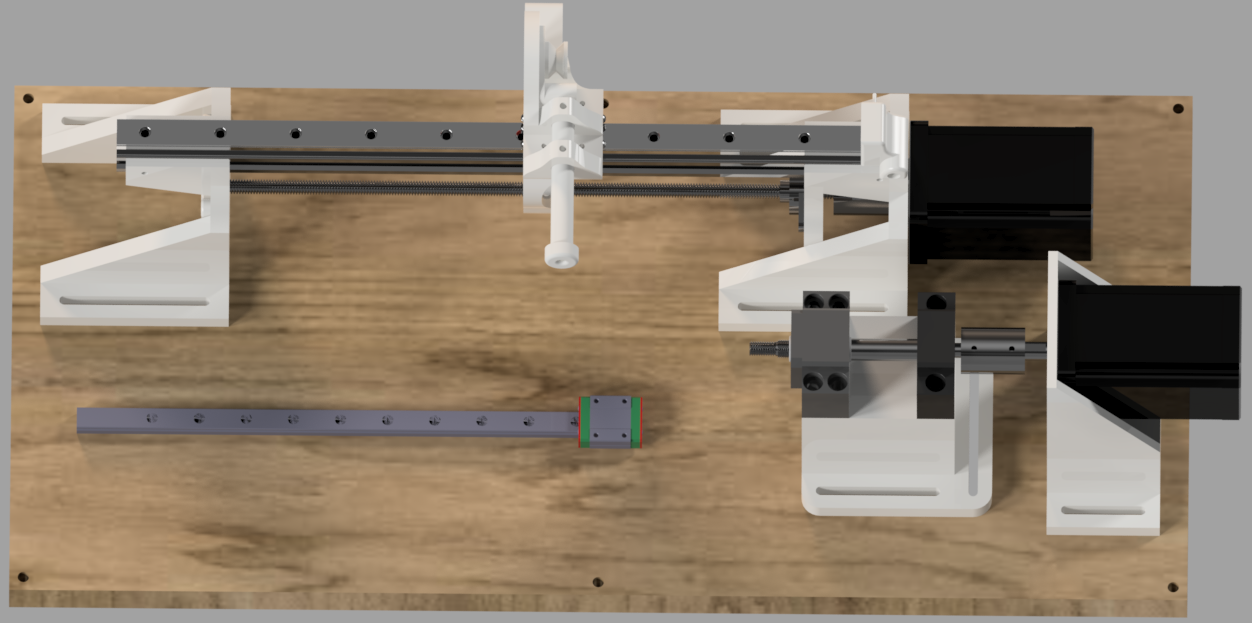
\includegraphics[width=0.25\textwidth]{./winder_render.png}
%     \caption{a nice plot}
%     \label{fig:winder_render}
% \end{figure}
% \begin{wrapfigure}{l}{0.35\textwidth}
%     \centering
%     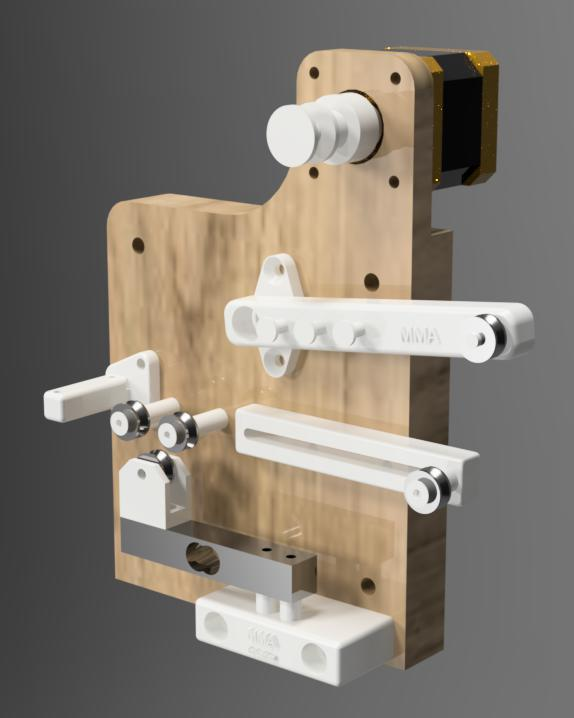
\includegraphics[width=0.35\textwidth]{./spannplatte_render.jpg}
% \end{wrapfigure}
Eine mögliche Erklärung für die, in (sie autoref{label}) ersichtliche, Geschwindigkeitsabhängigkeit der Drahtspannungskraft $\tau(v)$, bzw. Rückstellkraft $F_R(v)$, wäre, dass sich die Reibung an Filz !!!!!!!!!!!!! \newline
% Einfügen erklärung filz wie gas reibung und Erklärung kugellageröl viskosität


Für den nächsten Versuch wurden die selbe Wicklung, bei gleichbleibenden Wickelparametern, einmal mit Dancerarm und einmal ohne, je für beide Spulenkörper, durchgeführt. Der Draht wurde, bei nicht Verwendung des Dancerarms, direkt über das Kugellager der darunter liegenden Leiste geführt.


% \begin{figure}[H]
%     \centering
%     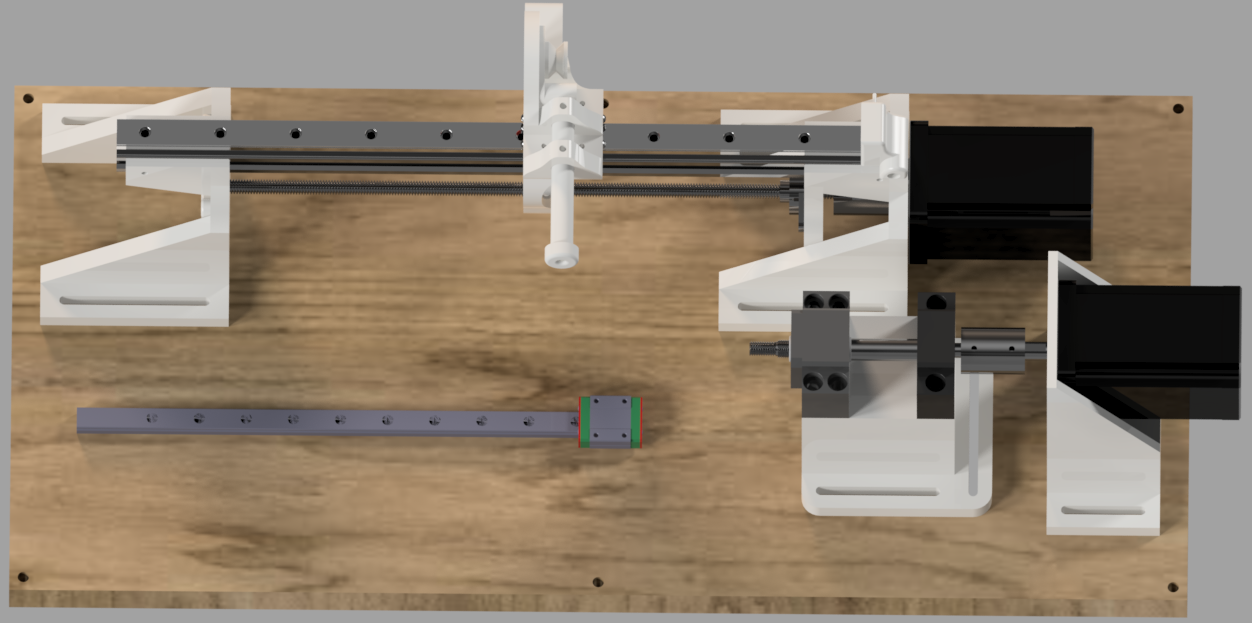
\includegraphics[width=0.25\textwidth]{./winder_render.png}
%     \caption{a nice plot}
%     \label{fig:winder_render}
% \end{figure}
% \begin{wrapfigure}{l}{0.35\textwidth}
%     \centering
%     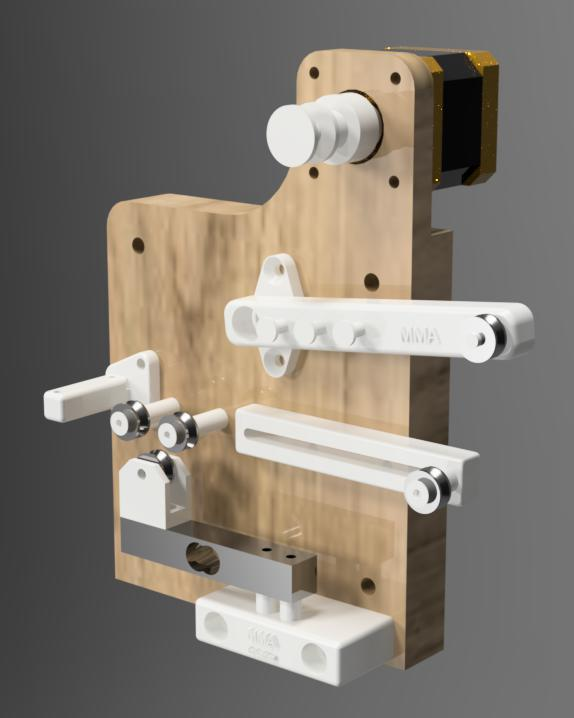
\includegraphics[width=0.35\textwidth]{./spannplatte_render.jpg}
% \end{wrapfigure}


% Text erklärung des Bildes



Zur Untersuchung der Start-, bzw. Abbremsphasen eines Wickeldurchganges sind in autoref{}!!!! die zwei Phasen, je für beide Spulentypen dargestellt. Die Messungen wurde jeweils mit der selben Beschleunigung und Endgeschwindigkeit durchgeführt.


% \begin{figure}[H]
%     \centering
%     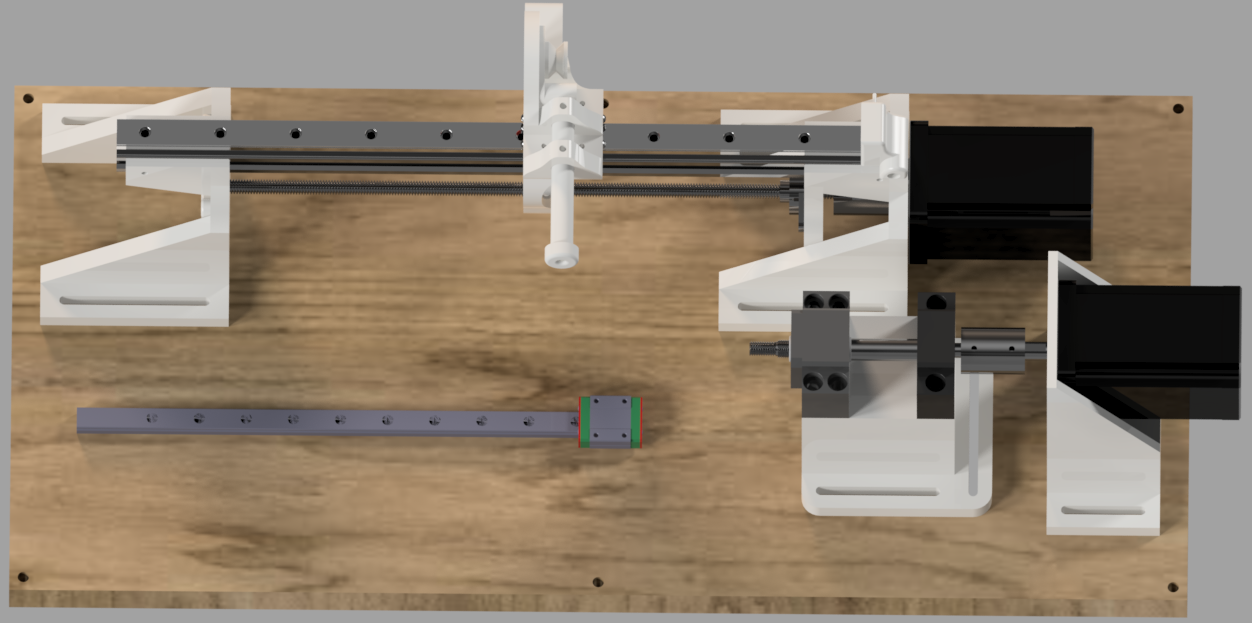
\includegraphics[width=0.25\textwidth]{./winder_render.png}
%     \caption{a nice plot}
%     \label{fig:winder_render}
% \end{figure}
% \begin{wrapfigure}{l}{0.35\textwidth}
%     \centering
%     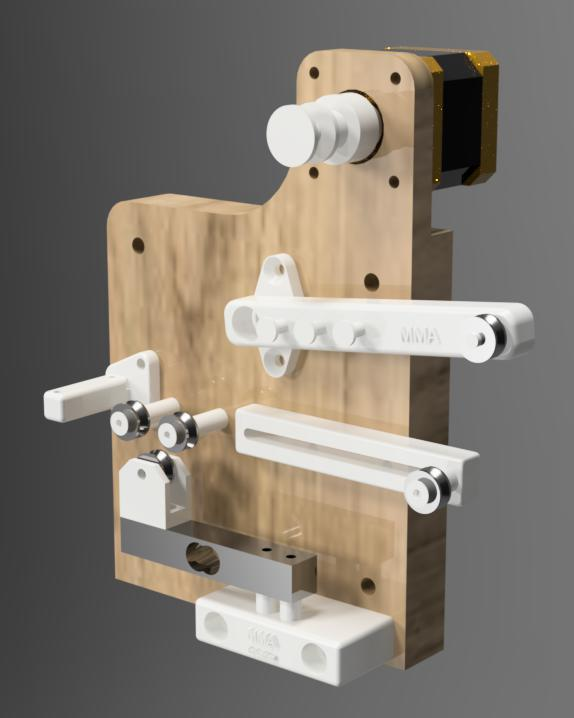
\includegraphics[width=0.35\textwidth]{./spannplatte_render.jpg}
% \end{wrapfigure}


% Text erklärung des Bildes





